The methods used in this study can be divided into water-related, energy-related and cost-related, with additional supporting processes (\fref{fig:framework}). GIS tools were widely used throughout the analysis, and a general model and case study runner for the NWSAS where developed using Python and hosted in a \href{https://github.com/camiloramirezgo/NWSAS-paper-model}{\textbf{Github repository}}.

\begin{figure*}[!h]
	\centering
	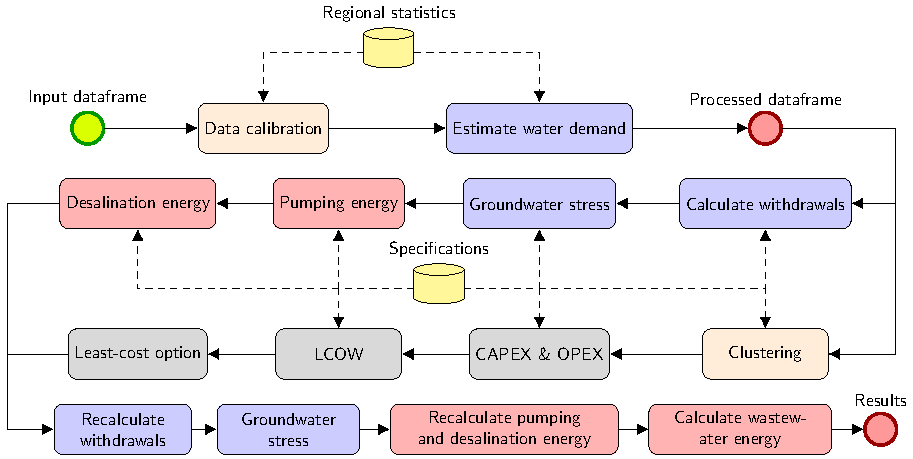
\includegraphics[width=\textwidth]{Framework}
	\caption{Methodology flow diagram---blue boxes indicate water-related methods, red boxes energy-related methods, gray boxes cost and LCOW related methods, orange boxes supporting methods and the yellow cylinders scenario characteristics data.}
	\label{fig:framework}
\end{figure*}

The analyzed system consisted of: extracting water from groundwater resources, desalinating brackish water when needed, supplying water demand for domestic and agricultural irrigation purposes, reclaiming domestic wastewater and agricultural drainage (i.e. tailwater), treating reclaimed wastewater, and reusing treated wastewater in agricultural irrigation. A schematic of the system is presented in \fref{fig:systemreuse}.

\begin{figure*}[!ht]
	\centering
	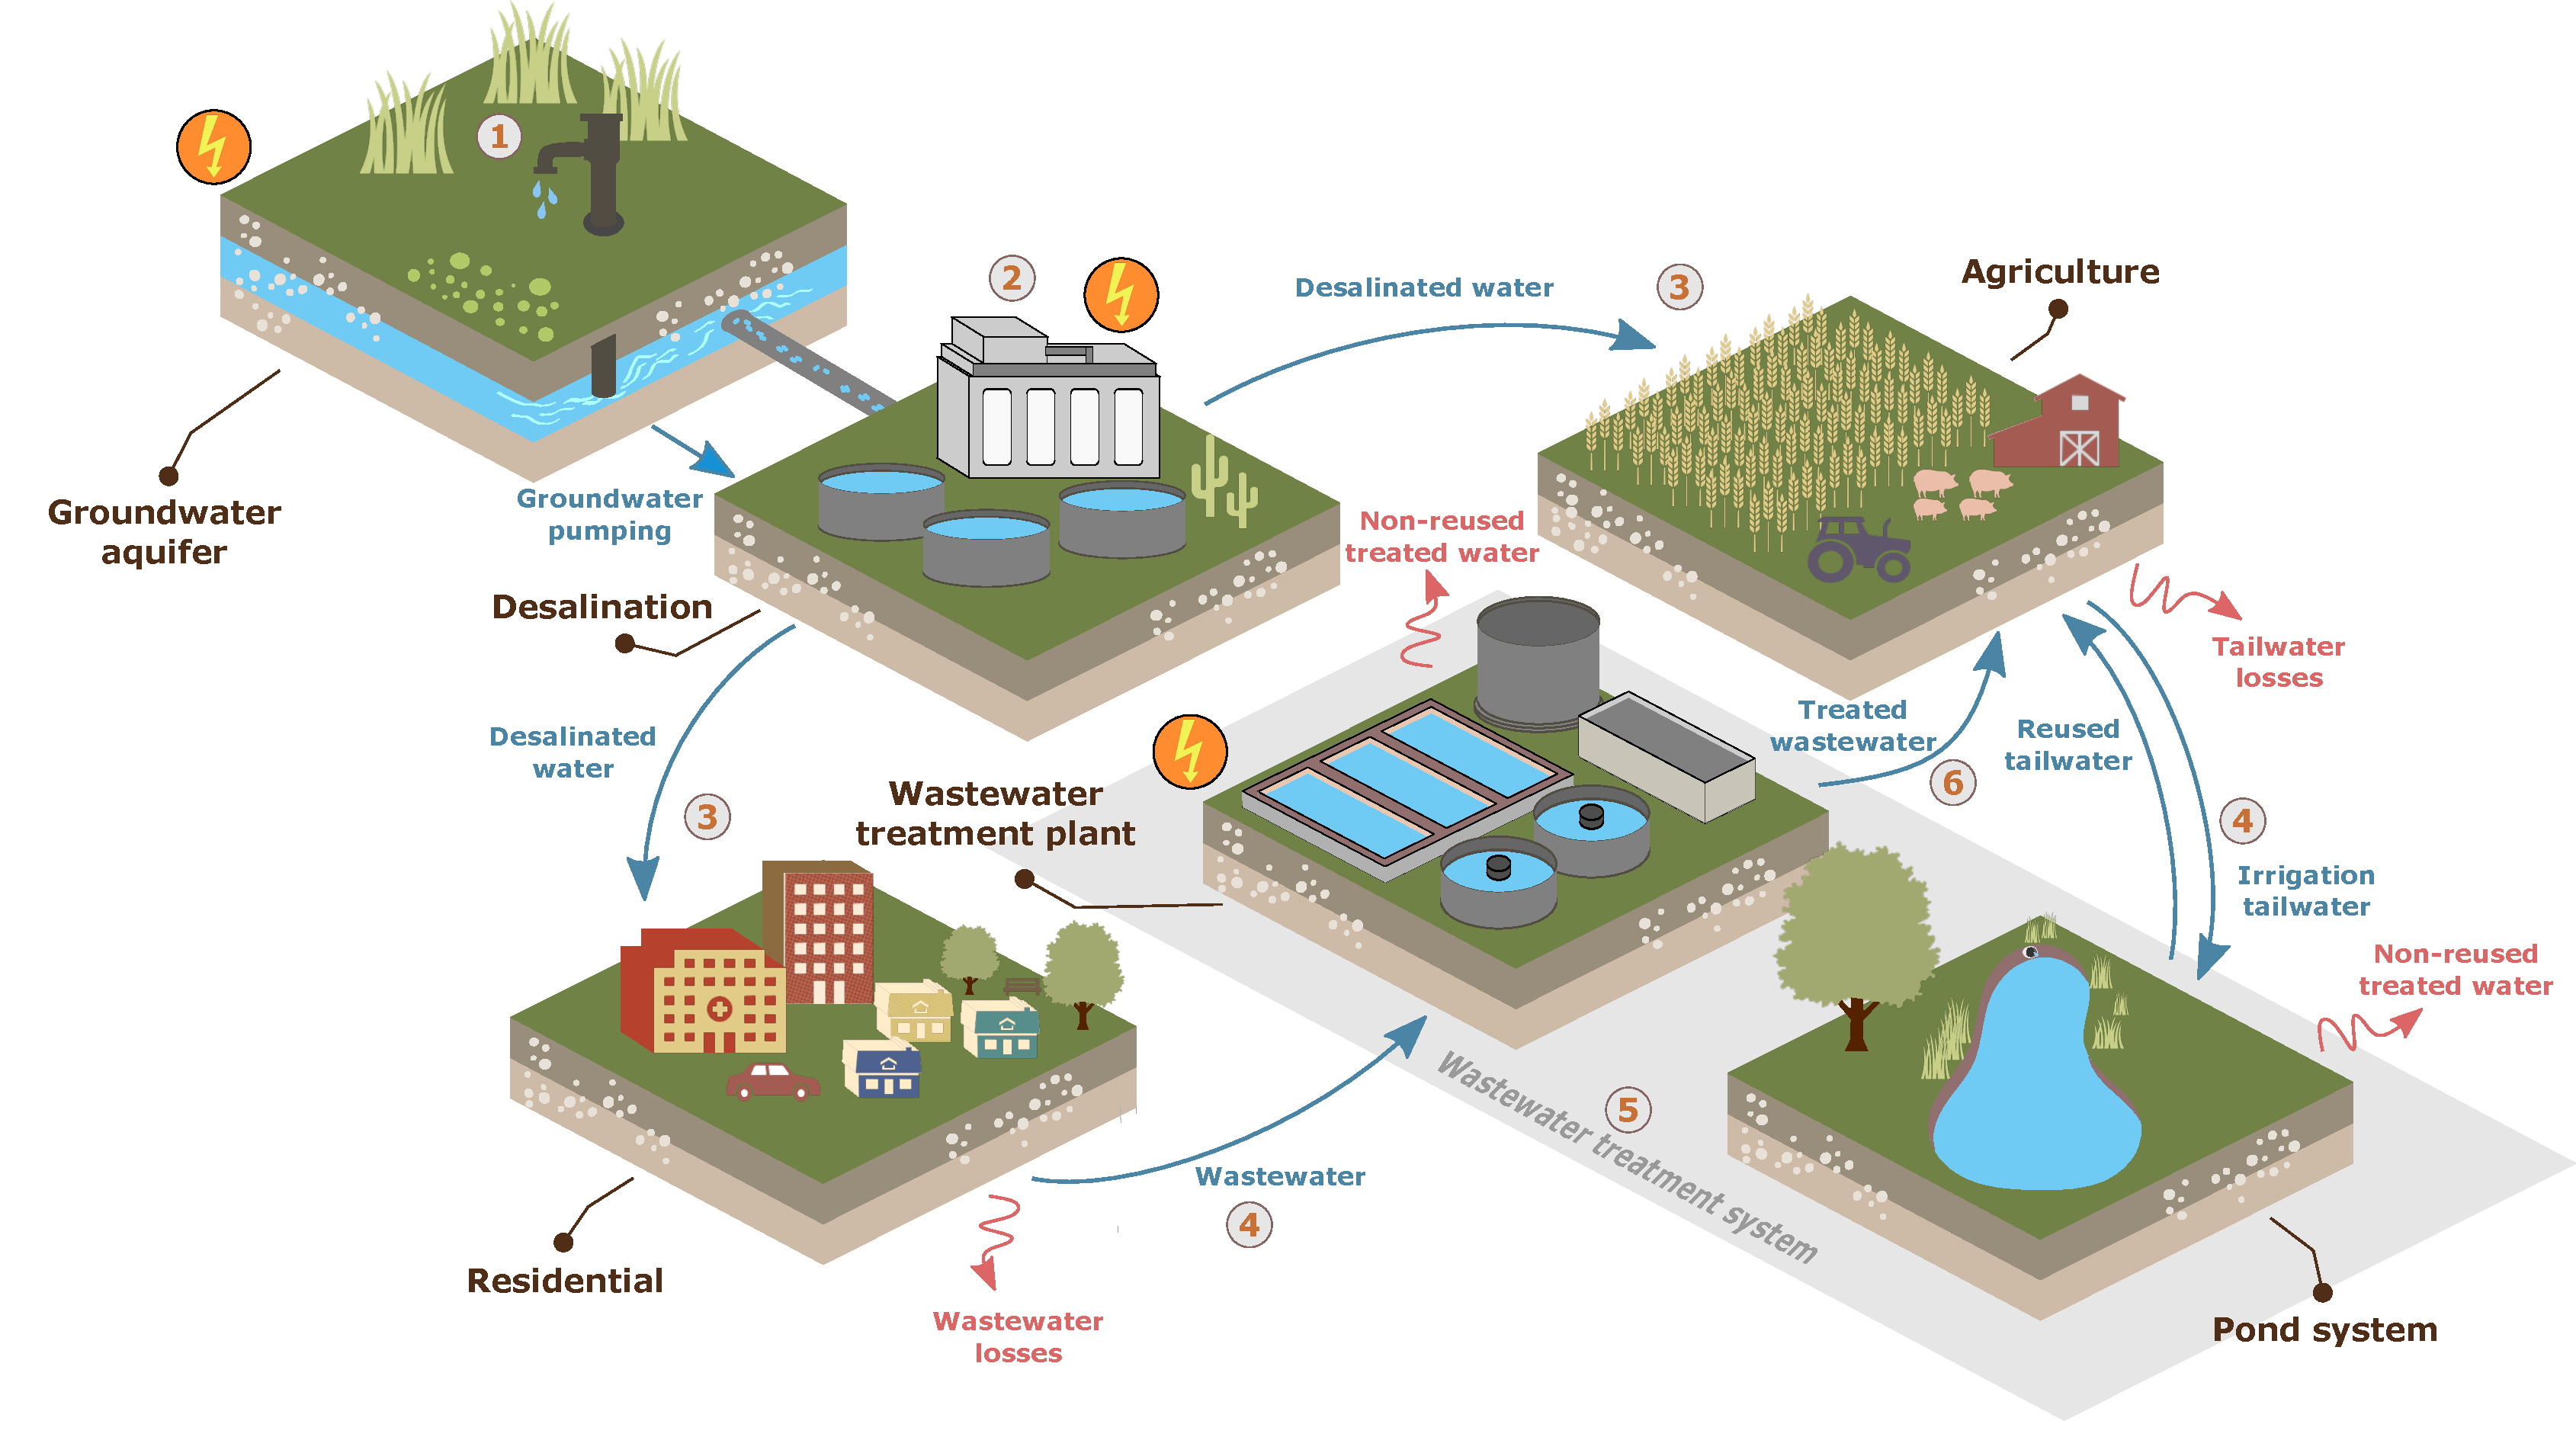
\includegraphics[width=\textwidth]{System_reuse}
	\caption{NWSAS components and resource streamflows - WWR scenarios.}
	\label{fig:systemreuse}
\end{figure*}

All water requirements for population consumption and agricultural irrigation were assumed to be supplied by the groundwater aquifer and that such water is desalinated whenever the TDS levels are above 1,000 mg/l \cite{fao1985water} (according to \textit{section 7} of the \textit{supplementary information}). Afterwards, the water is allocated for population consumption and agricultural irrigation. The recharge rate $R$ for the entire aquifer was taken as 1.1 billion cubic meters of water per year, which for the area of the aquifer, is an equivalent water column of 1.06 mm per year \cite{BetterValorizationIrrigation2015}. Furthermore, no environmental flow was considered.

Six wastewater treatment and reuse scenarios were analyzed, evaluating three irrigation water pricing regimes and two levels of population water consumption (see \tref{tbl:scenarios}). Irrigation water pricing regimes were taken from \cite{Socioeconomicaspectsirrigation2014}, were it was found that the irrigation water demand per hectare throughout the NWSAS basin is heavily dependent on the supply water cost. 

\begin{table*}[!ht]
    \caption{\label{tbl:scenarios}Scenario descriptions.}
	\footnotesize{
	\begin{tabular}{@{}l P{4.1in}}
		\br
		Scenario & Description\\
		\mr
		Baseline & The Baseline scenario is constructed with average yearly values of irrigation water consumption for each portion of the basin withing each country, being: Algeria 13,520 m\textsuperscript{3}/ha, Tunisia 13,266 m\textsuperscript{3}/ha and Libya 9,134 m\textsuperscript{3}/ha \cite{Socioeconomicaspectsirrigation2014}. Moreover, a low population water demand was used \cite{Householdwaterconsumption2014} (see below).\\
		Private agricultural water & Private farmers that pay the full price of water without any subsidy. The average level of water demand is around 10,512 m\textsuperscript{3}/ha \cite{Socioeconomicaspectsirrigation2014}. The \citet{Socioeconomicaspectsirrigation2014} found, that farmers belonging to this regime, have higher water productivity.\\ 
		Subsidized agricultural water & Users that have access to water subsidized to some extent. The average water demand is 15,334 m\textsuperscript{3}/ha \cite{Socioeconomicaspectsirrigation2014}.\\
		Free agricultural water & Farmers that have free access to water, meaning that the government fully subsidize the price of water and that the resource can be utilized without limitations. The average irrigation water demand is 21,215 m\textsuperscript{3}/ha \cite{Socioeconomicaspectsirrigation2014}.\\
		High population water & An average water consumption per capita of 73 m\textsuperscript{3}/year \cite{Householdwaterconsumption2014}.\\
		Low population water & An average water consumption per capita of 55 m\textsuperscript{3}/year \cite{Householdwaterconsumption2014}.\\
		\br
	\end{tabular}
	}
\end{table*}

It is worth noting that the large water demand increase seen in the subsidized and free regimes compared to the private regime, suggests a strong price elasticity of the irrigation water demand and/or the use of lower efficiency irrigation technologies in such regimes \cite{Socioeconomicaspectsirrigation2014}.

In addition, a sensitivity analysis was performed on the groundwater quality and depth to groundwater levels, in order to asses the impact they pose to the energy-for-water requirements (\tref{tbl:sensitivy}). This parameters were selected, as the water security of the aquifer highly depends on the water table levels and the quality of the resource, directly affecting food security as well.

\begin{table}[!ht]
	\caption{\label{tbl:sensitivy}Sensitivity parameters.}
	\begin{indented}
	\item[]\begin{tabular}{@{}l l l l}
		\br
		Parameter & Low & middle & high\\
		\mr
		Groundwater quality & -10 meters & current level & +10 meters\\
		Depth to groundwater & -50\% & current level & +50\%\\
		\br
	\end{tabular}
	\end{indented}
\end{table}

The most up-to-date open source data available was collected and processed using the open source software QGIS \cite{QGIS2020}. A data package comprising the geospatial characteristics of the study area was created, in order to capture key information to make the Nexus analysis possible. The relevant layers are identified and described in \textit{section 1} of the \textit{supplementary information}.

\subsection{Reclaimed wastewater and reused treated wastewater}
The amount of residential recoverable wastewater, was assumed to represent around 70\% of the total residential water consumed \cite{unescoWastewaterUntappedResource2017}. From that share, an additional 10\% was assumed to be lost in the capture, conveyance and treatment processes.
On the other hand, to evaluate the potential of capturing, storing and reusing irrigation tailwater, water requirements of the crops were estimated using the FAO-56 Penman-Monteith method for evapotranspiration \cite{allenFAOIrrigationDrainage1998}. Meteorological parameters were calculated from ``WorldClim" monthly data \cite{WorldClimGlobalClimate}  using the Python library ``Pyeto" \cite{pyeto}. For the purpose of this study, date palms were assumed to cover 100\% of the cropland area---as is one of the main crops cultivated in the region \cite{almullaNWSAS}. The crop coefficients and irrigation calendar were set according to \citet{almullaNWSAS}. From this process, the yearly crop water needs throughout the entire basin were obtained.

Furthermore, an on-farm storage pond system was evaluated to account for the potential reusable water. For this, a water balance on the on-farm storage was executed following a similar approach to \citet{reinhartSimulatedWaterQuality2019}. First, the maximum attainable irrigation efficiency (i.e. crop water requirements over irrigation water applied) was set to be 80\%, being the remaining 20\% non-recoverable loses. If additional water was available, it was recovered and stored. The storage reservoir surface area, was assumed at 2\% of the cropland area and a standard depth of 3 meters \cite{reinhartSimulatedWaterQuality2019}. Leakage losses in the storage system were set to be 0.9 mm/day, and evaporation loses were calculated using a modified Penman-Monteith method for an open water body \cite{reinhartSimulatedWaterQuality2019}. For this, and albedo, surface height, and surface roughness values of 0.05, 0.002 m, and 0 s/m, respectively were used \cite{princeczarneckijobym.QuantifyingCaptureUse2017}.

\subsection{Groundwater Stress Indicator}
The Groundwater Stress Indicator was used to quantify the current stress of the aquifer \cite{Aqueductglobalmaps2015}. It relates the ratio of water withdrawals due to anthropogenic reasons (e.g. potable water, industrial water, recreational water, irrigation water, etc.), and the total recharge rate of the aquifer (subtracting the environmental stream flow). The groundwater stress indicator is usually calculated as the ratio of groundwater footprint to aquifer area \cite{RegionalGroundwaterStress2013}.

\subsection{Clustering algorithm}\label{Sc:clustering}
A clustering approach was used in order to identify dense areas where a wastewater treatment system could be implemented, minimizing constraints imposed by existent large distances among scatter population or irrigated lands. A hierarchical clustering  algorithm was run using the \textit{Agglomerative Clustering} object from the Python \textit{scikit-learn} package \cite{scikit-learn}.

\begin{figure*}[!b]
    \centering
	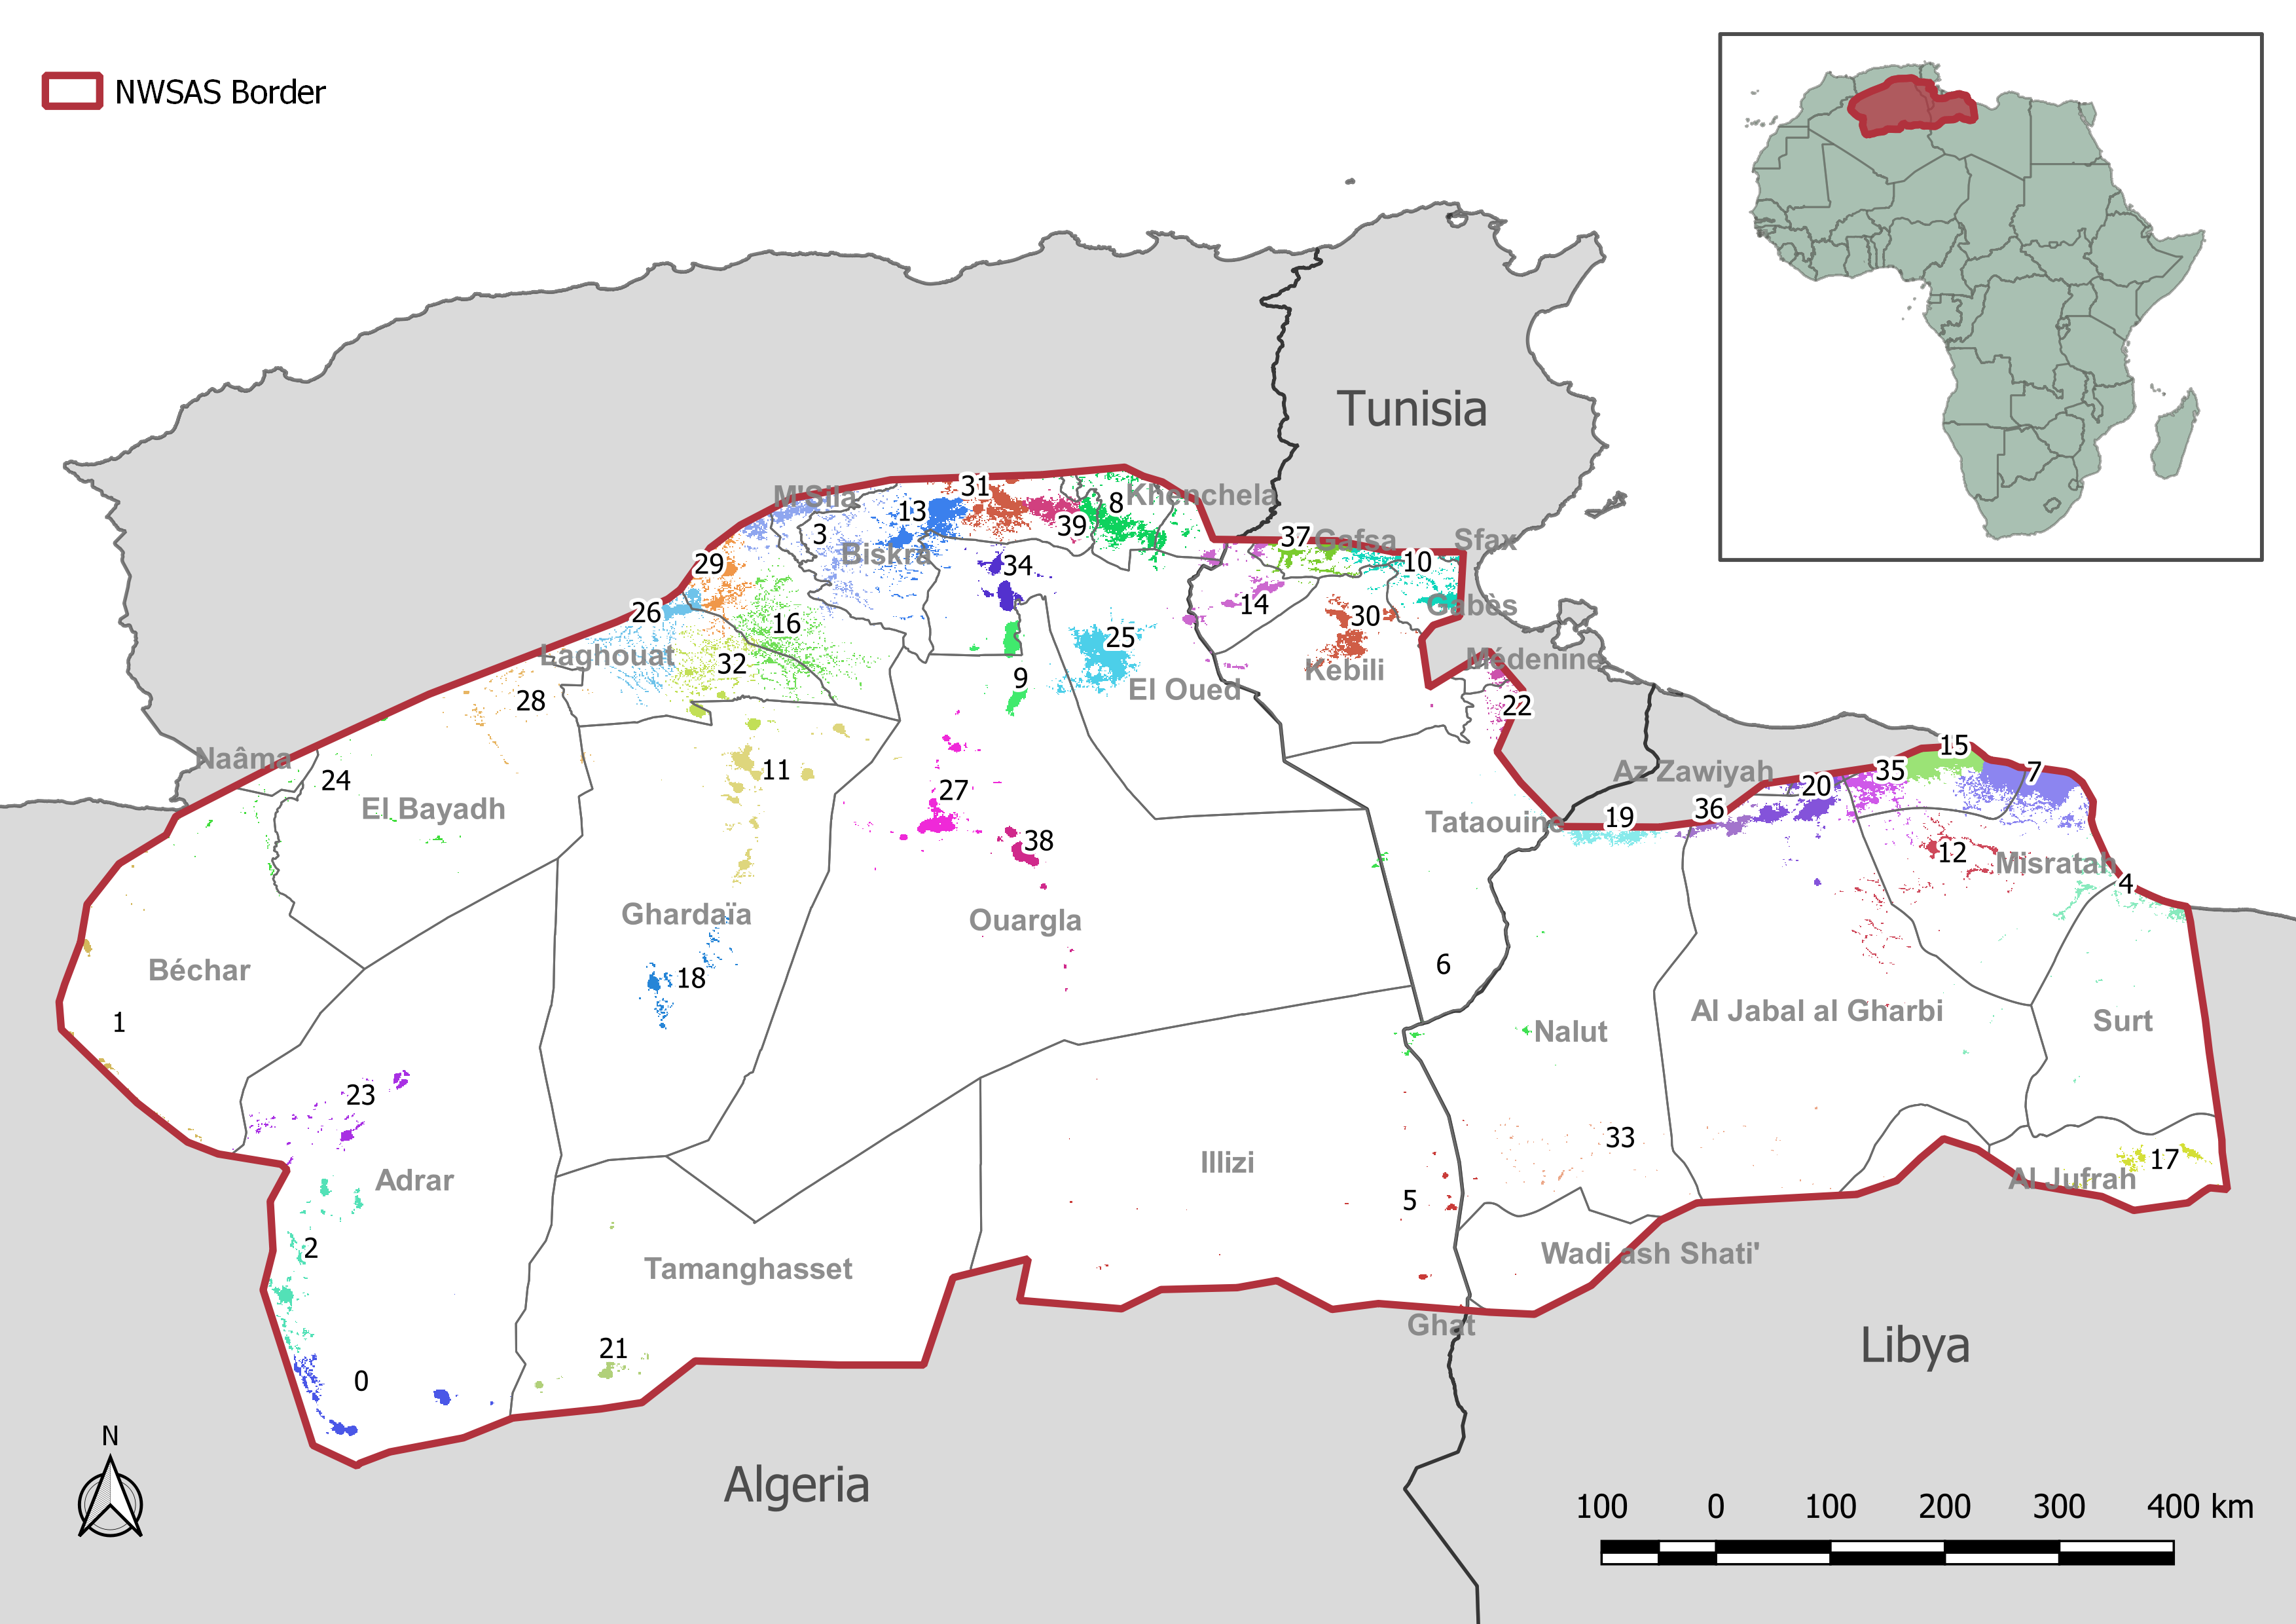
\includegraphics[width=0.88\textwidth, cfbox=black 1pt 0pt]{NWSAS_clusters}
	\caption{Population and cropland clusters. Clusters are numbered from 0 to 39, yielding 40 agglomerations including each population and cropland areas. Every cluster is tagged with a number and colored to make them stand out from others. The grey administrative boundaries correspond to the different provinces.}
	\label{fig:clusters}
\end{figure*}

Forty clusters were created (\Fref{fig:clusters}) in the process, which succeeded in identifying dense agglomerations. When compared with a traditional approach of performing an analysis on a province basis, the clusters achieved a reduction of 347\% on the overall distance between points.

This is especially important in larger provinces with substantial population and agricultural activity as Adrar, Ghardaïa, Ouargla el Oued and Misratah. Moreover, with this approach, the administrative border constraint is eliminated, as can be seen with cluster number 9 where the agglomeration shares areas from the Ouargla and El Oued provinces.

\subsection{Wastewater Treatment System characteristics}
Wastewater pollutant levels, were assumed to be constant throughout the basin, using standard values based on studies from FAO \cite{fao1985water}. The assumed pollutant levels for population wastewater and the required levels for reused treated wastewater, are shown in \textit{section 6} of the \textit{supplementary information}.

Cost functions were used to estimate CAPEX and OPEX values for the different Wastewater Treatment Technologies (WWTTs), as statistical methods have shown to be commonly used in cost-modelling for wastewater management \cite{Costmodellingwastewater2011,Assessmentwastewatertreatment2012,Economicfeasibility2012}. However, technology specific cost functions were not available for the NWSAS basin area, nor statistical data to develop them. Therefore, based on the work of \citet{Assessmentwastewatertreatment2012} cost functions for different WWTT in Spain were used to evaluate the competence of selected technologies in the NWSAS (see \textit{section 6} of the \textit{supplementary information}). Energy intensity characteristics were added for each technology according to \cite{Energypatternanalysis2012,ComparativeAnalysisEnergy2017}.

\subsection{Levelized Cost of Water}
A proposed LCOW method was used as a metric to compare cost-effectiveness among WWTTs. The LCOW assesses the life-cycle cost of delivering one unit (e.g. one cubic meter) of treated wastewater, based on all physical assets and resources required. This concept, is inherited from the Levelized Cost of Electricity (LCOE) methodology, which applies the same life-cost analysis for one unit of electricity output \cite{prospectscostcompetitive2013}. The LCOW method follows the logic of the LCOE method \cite{prospectscostcompetitive2013,GeospatialLevelizedCost2015}, with pertinent adjustments to the variables used in wastewater treatment systems. The project life span was set for 35 years, covering the period from 2015 to 2050. Then, the LCOW can be expressed as follows:

\begin{equation}\label{eq:lcow}
LCOW = LCOW_{Inv} + LCOW_{O\&M} + LCOW_{Ext}
\end{equation}

The expression presented in \eref{eq:lcow}, disaggregates the $LCOW$ (\$/m\textsuperscript{3}) value in three components: the cost components due to investment $LCOW_{Inv}$, operation and maintenance $LCOW_{O\&M}$ and externalities $LCOW_{Ext}$. As the CAPEX function comprises all investment components of a wasteater treatment plant, it enables an easy calculation of the $LCOW_{Inv}$ for each WWTT and each region or cluster. \Eref{eq:lcowinv} describes the process to calculate the $LCOW_{Inv}$.

\begin{equation}\label{eq:lcowinv}
LCOW_{Inv} = \frac{Inv}{\sum_{t=1}^{T} V_{t}\cdot\gamma^{t}}\cdot\Delta
\end{equation}

Where $Inv$ stands for the CAPEX value, $V_{t}$ for the treated water flow per year $t$ (m\textsuperscript{3}/yr), $\Delta$ for the tax factor and $\gamma^{t}$ represents the discount factor of the project (see section 8 of the \textit{supplementary information}).

The LCOW related to operational costs $LCOW_{O\&m}$ \eref{eq:lcowom} was computed by using the OPEX values $\omega_{t}$ calculated for each year in each cluster, the treated water flow $V_{t}$ (m\textsuperscript{3}/yr) and the discount factor $\gamma^t$ per year.

\begin{equation}\label{eq:lcowom}
LCOW_{O\&m} = \frac{\sum_{t=1}^{T} \omega_{t}\cdot V_{t}\cdot\gamma^{t}}{\sum_{t=1}^{T} V_{t}\cdot\gamma^{t}}
\end{equation}

Furthermore, the avoidance of externalities due to discharge of untreated wastewater into ecosystems, can be accounted by estimating the effects that pollutants presented in wastewater and tailwater stream flows can have into fresh water bodies, rivers or groundwater aquifers (see section 8 of the \textit{supplementary information} for more detail) \cite{Assessmentwastewatertreatment2012}. However, due to lack of information of environmental effects of wastewater pollutants in the region, this parameter was not considered.